% Please do not delete!  thanks! -- zach
% !TEX root = ../../main.tex

\section{Evaluation}
In this section, we present the evaluations that been performed on our solutions. This including two parts: 1) methods that used to evaluate our core topic learning models LDA and Doc2Vec and 2) methods used to evaluate the whole solution as the final product. 
\subsection{Evaluating Learning Models}
The performance measure is a typical way to evaluate machine learning models. It is the measurement that will make of the predictions made by a trained model on the test dataset. Performance measures are typically specialized to the class of problem, for example in this paper, while we using LDA  to deal with NLP topic modeling, we will use likelihood score and clustering result to evaluate our LDA model.\\
Based on how to split the data into training and testing, evaluate machine learning models usually involves hold out, cross validation(CV) and leave-one-out. \\
Hold out method is a simple split of dataset, for example, 70\% of the instances are used for training the models, the rest 30\% for testing the model. In the CV method, it first involves separating the dataset into a number of equally sized groups of instances (called folds). The model is then trained on all folds exception one that was left out and the prepared model is tested on that left out fold. The process is repeated so that each fold get's an opportunity at being left out and acting as the test dataset. Finally, the performance measures are averaged across all folds to estimate the capability of the algorithm on the problem.  Leave-one-out is a special case of CV, where folds is equal to data points.\\
In our original plan, we may need CV to run our model evaluation, because our dataset is not large enough and the computational difficult is not critical. But with using only stackoverflow data, we have plenty of dataset. So the decision is using hold out method. We tested our models using different size of dataset. 
\paragraph{Dataset Description} 
Ultimately, we plan to use actual open source books as our primary dataset, which including over 100 books in computer science discipline. As our work went through, we plan to use some other dataset that have pre-labeled topics to train our models as the risk reduction process. With this in mind, we download stackoverflow posts data. The original posts data is in xml format, about 62G Bytes. Each post contains post body, post tag, post time and other attributes.
\paragraph{Data preparation} 
StackOverFlow dataset is a signal file in xml format. In order to use these data to train our models, we need to do some data preprocessing to clean up the data. In the topic modeling, the input data is text itself, which is post body in the case of stackoverflow dataset. After training, during the test phase, the extracted topics from the test dataset using the trained model, will be compared with the actual topics, which are the post tags. In summary, the first step of data preparation is to extract post body and tags from raw data.\\
Normally, with the text corpus ready, the next data preprocessing would be removing punctuations in the text corpus, and changing words to lower cases, but these steps have been included in our models. So the input to models are the parsed post body text files.
\paragraph{Evaluating LDA}
One typical method to evaluate LDA model is to calculate the likelihood probability of the testing data(hold out data in our case). We used perplexity to calculate and estimate the likelihood. Perplexity is defined as the reciprocal geometric mean of the token likelihoods in the test text corpus given the trained model. Lower values of perplexity means lower misrepresentation of the words of the test files by the trained topics. 

\paragraph{Evaluating Doc2Vec}
TO DO

\paragraph{Sentiment Prediction Accuracy}
%Need to figure out how to test the accuracy of doc2vec when it predicts future text
%
%-gensim has a infer vector function that "infers a vector for given post-bulk trainng document"
%
%-calling model.docvec[doc tag/id] should pull up the vectors that were trained already
%	-I think gensm uses most similar function to find a good trained vector (good because it would predict the given document well)
%	- so if the most similar trained vector is very different than the infered vector, the model is not good?
%
%-I suppose we should be infering documents that were not used in training
%
%-Error rate would be how far away best vectors are, lower the better?

\paragraph{Information Retrieval}

One way to verify that our implementation of Doc2Vec is correctly mapping word vectors to other semantically similar word vectors is to test the trained model on an information retrieval task . \cite{RefWorks:doc:5a6e5746e4b0d609eec798d7} The data collected from stackoverflow is tagged with different topics that pertain to the content. The tags can then be used to organize the content via topic. The Doc2Vec model should report two documents that pertain to the same topic as less distant to each other than a third document that focuses on a different topic.

%-Seperate content such that documents used for testing were not trained on
%
%- 3 folders: two with the same topic, a third folder of different topics that don't include the picked special topic
%-Report results (use DM, DBOW, and both together -follow gensim example at https://github.com/RaRe-Technologies/gensim/blob/develop/docs/notebooks/doc2vec-IMDB.ipynb 
\subsection{Evaluating Application}
\paragraph{Pre-Surveying}
To evaluate our project idea, we conducted a pre-surveying to see what the problem we are facing and how people reacting about our proposed solution. We asked our participants how long they will spend on find the right textbook, what aspect do they think is most important when choosing a textbook (except the content, our learning model will do the best of this part). See Table \ref{Pre-survey} for a breakdown of the questions to ask.

\begin{tabular}{ll}
\multicolumn{1}{c}{\bf Questions in Pre-Survey} 
\\ \hline \\
1. Are you a student or professor?\\
2. How much time do you spend on choosing a textbook?\\
3. How do you choose a textbook?\\
4. What aspect do you think is most important\\
when choosing a textbook (except the content)? \\
5. Would you consider an app that will give you \\
recommended textbooks base on your course \\
syllabus and your preference? \\
\end{tabular} \label{Pre-survey}

Among the 29 responses, we found that 73.3\% responded as they interested to our application to recommend the textbooks. The answer to most important aspect during the textbook chosen, review/ratings and sell price were the highest concern. These preliminary results give us the guidance to design the application and to improve the core learning models. See Figure \ref{result_of_presurvey} for detailed results.

\begin{figure}[ht]
\caption{Result of preSurvey}
\label{result_of_presurvey}
\centering
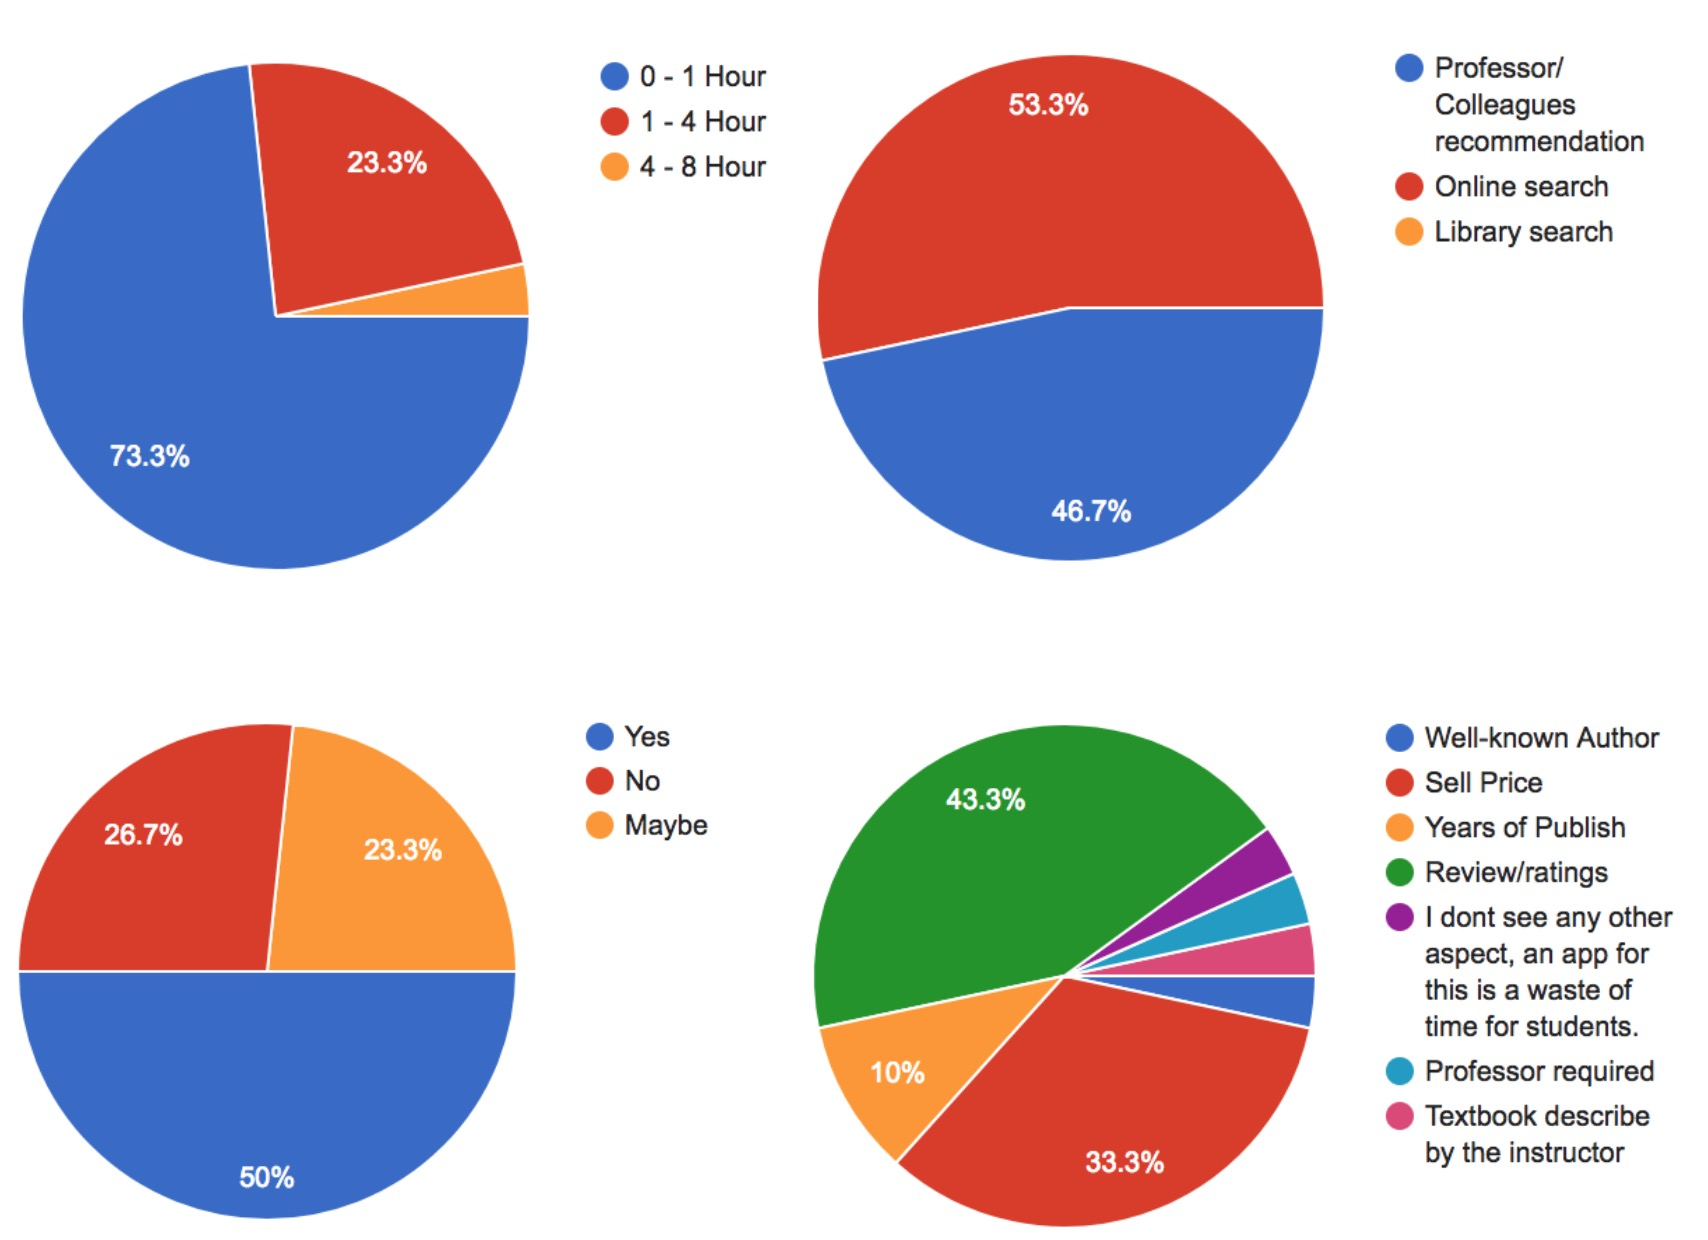
\includegraphics[width=0.5\textwidth]{preSurvey.jpeg}
\end{figure}

\paragraph{Experiments and Post-survey}
After we build the application with the command line interface and core learning models, we ran the experiments with different users in a foucs group to evaluate the solution.

%%% Local Variables:
%%% mode: latex
%%% TeX-master: "../../main"
%%% End:
